\section{The Hierarchical Poincaré-Steklov Method}

Initial work towards a fast, direct solver for elliptic PDEs is somewhat inspired by advances in fast algorithms for boundary integral methods. These kind of algorithms include fast multipole methods, panel clustering, wavelets, etc. \cite{martinsson2004fast}. Motivation for a fast, direct solver (vs. an iterative one) stems from wanting to improve upon the disadvantages of iterative solvers, namely from \cite{martinsson2004fast}:

\begin{adjustwidth}{0.25cm}{}
    1) The number of iterations for convergence is sensitive to the spectral properties of the matrix $\textbf{A}$. In many cases, $\textbf{A}$ can be ill-conditioned and convergence is very slow.

    \noindent 2) Iterative methods can only be applied to one problem at a time, whereas a direct inversion (or factorization) of $\textbf{A}$, once built, can be applied to as many RHS as desired.

    \noindent 3) Iterative methods for linear systems with "close" matricies cannot take advantage of the closeness of the matricies, whereas direct methods could (i.e. if we have an inverse or factorization of $\textbf{A}$ and perturb it by $\epsilon$, we could adjust the inverse to account for it instead of recompute the inverse.)

    \noindent 4) Most direct methods can take advantage of fast and efficient algorithms for matrix factorization such as the singular value decomposition, LU-decomposition, QR-decomposition, etc.
\end{adjustwidth}

The work done by Martinsson and Gillman in \cite{martinsson2004fast}, \cite{MARTINSSON2013460}, and \cite{gillman2014direct} (with a great tutorial found in \cite{martinsson2015hierarchical}) culminate in what they call the Hierarchical Poincaré-Steklov (HPS) method. It is a direct solver for elliptic PDEs that is based on a hierarchical binary tree of rectangular patches where the solution operator to $\textbf{A}$ is built by recursively merging child patches.

\subsection{Overview of the Hierarchical Poincaré-Steklov Method}

We'll provide a high level overview of the HPS method, following steps from \cite{gillman2014direct} and \cite{martinsson2015hierarchical}. The method can be broken into a build stage (which involves leaf operations and a merge step) and a solve stage.

\subsubsection{Build Stage: Leaf Level Computations}

In the build stage, the goal is to build and store an in-memory solution operator from merging children patches. Start with the parent level domain, or the domain of the original problem. Decompose the domain by splitting the domain in half to form two children patches. Continue splitting each patch in half (horizontally and then vertically, or vice versa, it doesn't matter) until a user-defined precision or level of refinement is reached. This forms the binary tree of rectangular patches. The lowest level patches are called leaf patches. This procedure is outlined in Figure \ref{fig:build}.

\begin{figure}
    \centering
    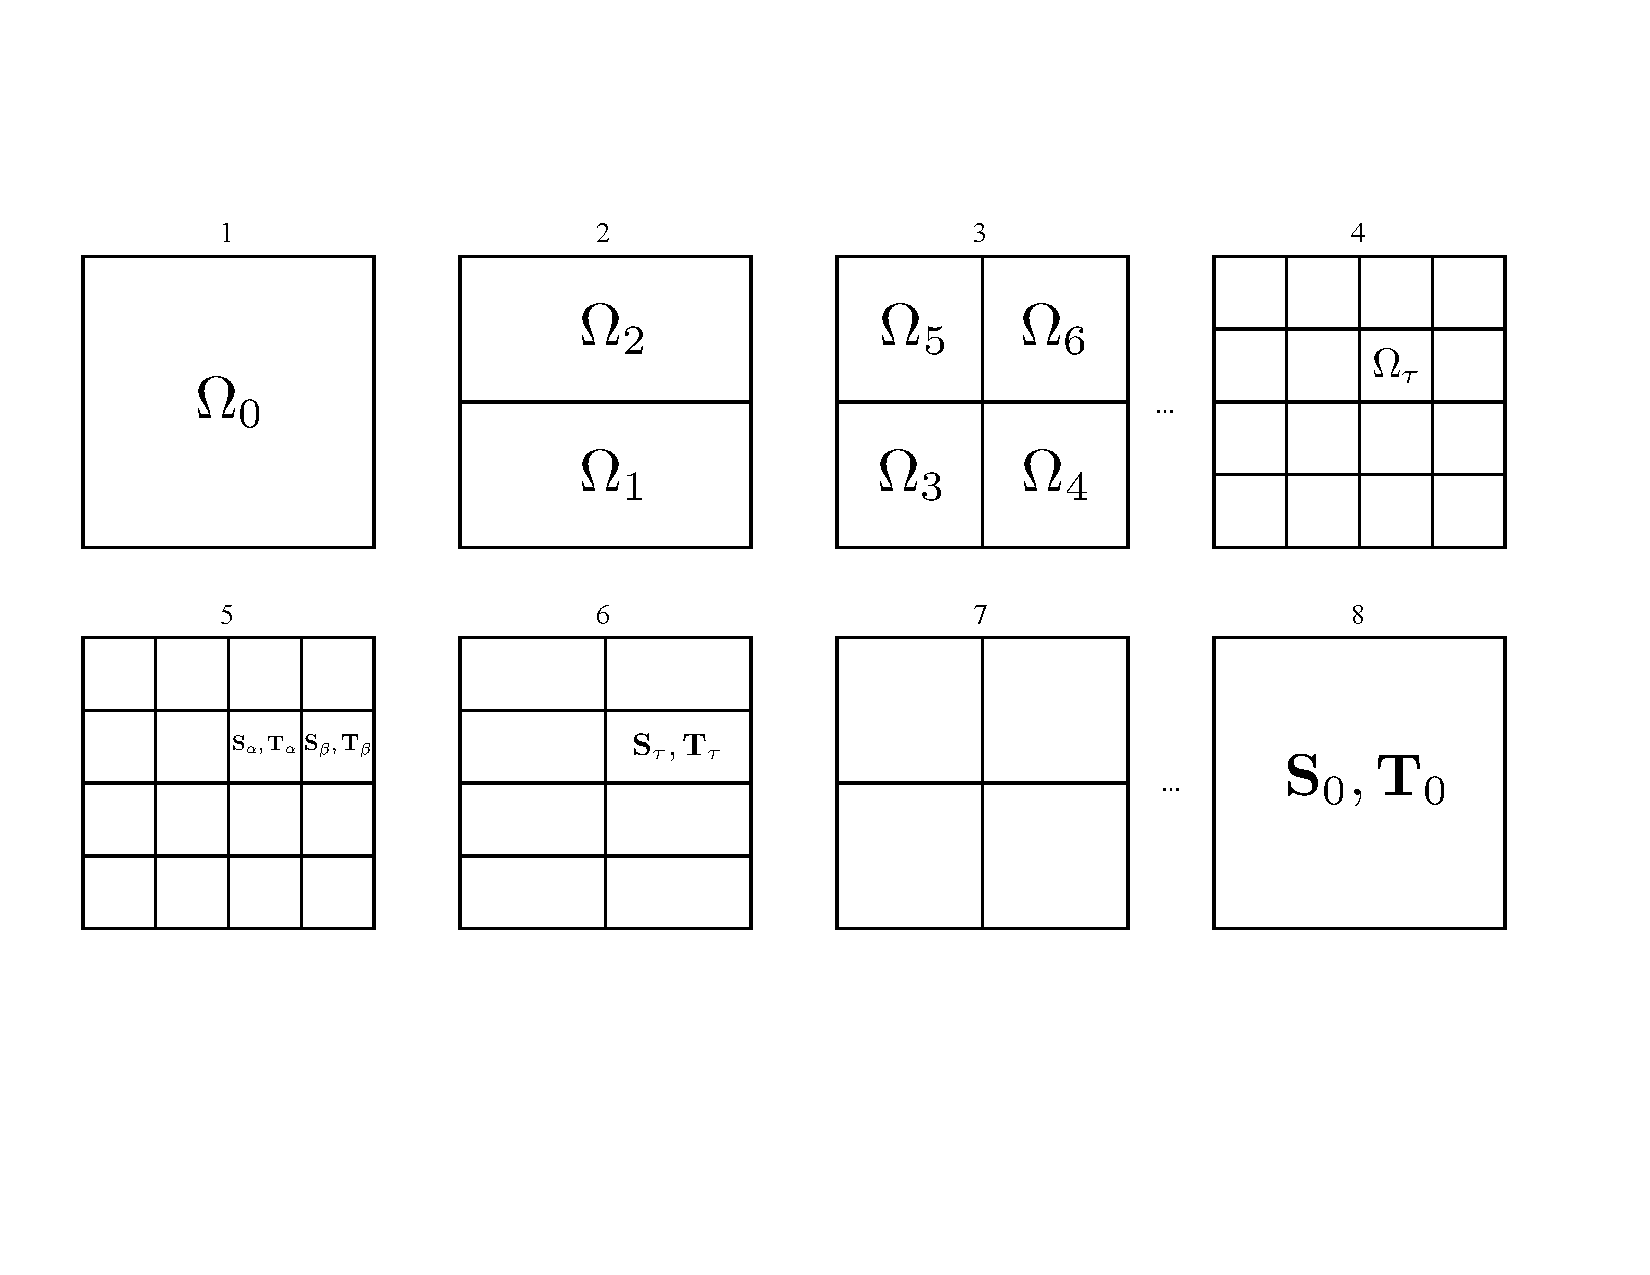
\includegraphics[width=\columnwidth]{figures/build_figure.pdf}
    \caption{The HPS Build Stage. Steps 1-3 show the domain decomposition into a hierarchical tree of rectangular patches. Step 4 shows the continued decomposition until a desired precision or refinement. Step 5 shows the leaf level solution operators $\textbf{S}_{i}$ and DtN operators $\textbf{T}_{i}$. Step 6 shows the merged operators from children $\Omega_{\alpha}$ and $\Omega_{\beta}$ to parent patch $\Omega_{\tau}$. Steps 7-8 show this continued to the top of the tree.}
    \label{fig:build}
\end{figure}

On the leaf level, the next task is to build the local solution operator $\textbf{S}$ and local Dirichlet-to-Neumann operator $\textbf{T}$. The solution operator $\textbf{S}$ maps Dirichlet boundary data to solution data on the interior
\begin{align}
    \textbf{S} \textbf{g} = \textbf{u}_{int}.
\end{align}
In other words, the solution operator solves the local BVP as soon as it has the required boundary information. In order to define the DtN operator, we first define Neumann flux data on the boundary of a patch domain as
\begin{align}
h(\textbf{x}) = \frac{\partial u(\textbf{x})}{\partial n} \Big|_{\textbf{x} \in \partial \Omega_{\tau}}
\end{align}
and define the vector $\textbf{h}$ to be the Neumann data sampled at the boundary points. Then, the Dirichlet-to-Neumann operator maps Dirichlet data on the boundary to Neumann data on the boundary
\begin{align}
    \textbf{T} \textbf{g} = \textbf{h}.
\end{align}

The DtN operator falls under a broader category of operators called Poincaré-Steklov operators, which the interested reader can learn more about in \cite{quarteroni1991theory}.

In order to compute leaf level operators as defined above, Martinsson in \cite{martinsson2015hierarchical} and Gillman in \cite{gillman2014direct} both use a spectral decomposition of Chebyshev and Gaussian nodes. They use map between Chebyshev and Gaussian nodes at different points to take advantage of each sets' respective advantages. Spectral differential techniques all Martinsson and Gillman to explicitly define $\textbf{S}$. Additional ways to form $\textbf{S}$ depend on the type of discretization on the leaf level patches. For example, if instead of a tensor product of Chebyshev ndoes, a user discretizes a leaf patch with a finite volume grid, the solution operator would be derived from a stencil matrix as in \cite{leveque2007finite}.

Another approach to ``building" $\textbf{S}$ is to actually not build $\textbf{S}$, but have a function that applies the operation of the solution operator. In practice, any iterative or direct method to solve an ellipitc BVP would work. The goal is to have a function that takes grid information and the Dirichlet boundary data and outputs the solution data on the interior.

Next, we look at how to compute the DtN operator $\textbf{T}$ on the leaf level. Martinsson and Gillman do this through a retabulation of Gaussian to Chebyshev nodes, apply the solution operator, perform a spectral differentiation in the normal direction to obtain flux data, and then retabulate back to Gaussian nodes. In practice, this looks like a product of four linear operators. Considering other methods, if a user has a way to apply the solution operator, one can form $\textbf{T}$ by iterating through the columns of the identity matrix applied to the solution operator. This could also take advantage of the structure of $\textbf{T}$. Efforts to find different ways to form the DtN operators are ongoing.

\subsubsection{Build Stage: Merging Operators}

Once all of the leaf level computations are done, the next step is to merge neighboring patches in an upwards pass of the tree. The merge process can be thought of as an elimination of the nodes on the interface of two patches. This takes the form of a Schur complement for a blocked system comprised of indexed boundary nodes.

We will use the notation from \cite{martinsson2015hierarchical} and \cite{gillman2014direct} to express the merged operators. We define the following index sets:
\begin{align*}
    \textbf{I}_1 &= \text{Boundary nodes of } \alpha \text{ that are not boundary nodes of } \beta \\
    \textbf{I}_2 &= \text{Boundary nodes of } \beta \text{ that are not boundary nodes of } \alpha \\
    \textbf{I}_3 &= \text{Boundary nodes of } \alpha \text{ and } \beta \text{ that are not boundary nodes of the union of } \alpha \text{ and } \beta
\end{align*}
Figure \ref{fig:merge} shows the merged patch $\tau$, with children $\alpha$ and $\beta$. The red nodes correspond to $\textbf{I}_1$, the green nodes correspond to $\textbf{I}_2$, and the blue to $\textbf{I}_3$.

\begin{figure}
    \centering
    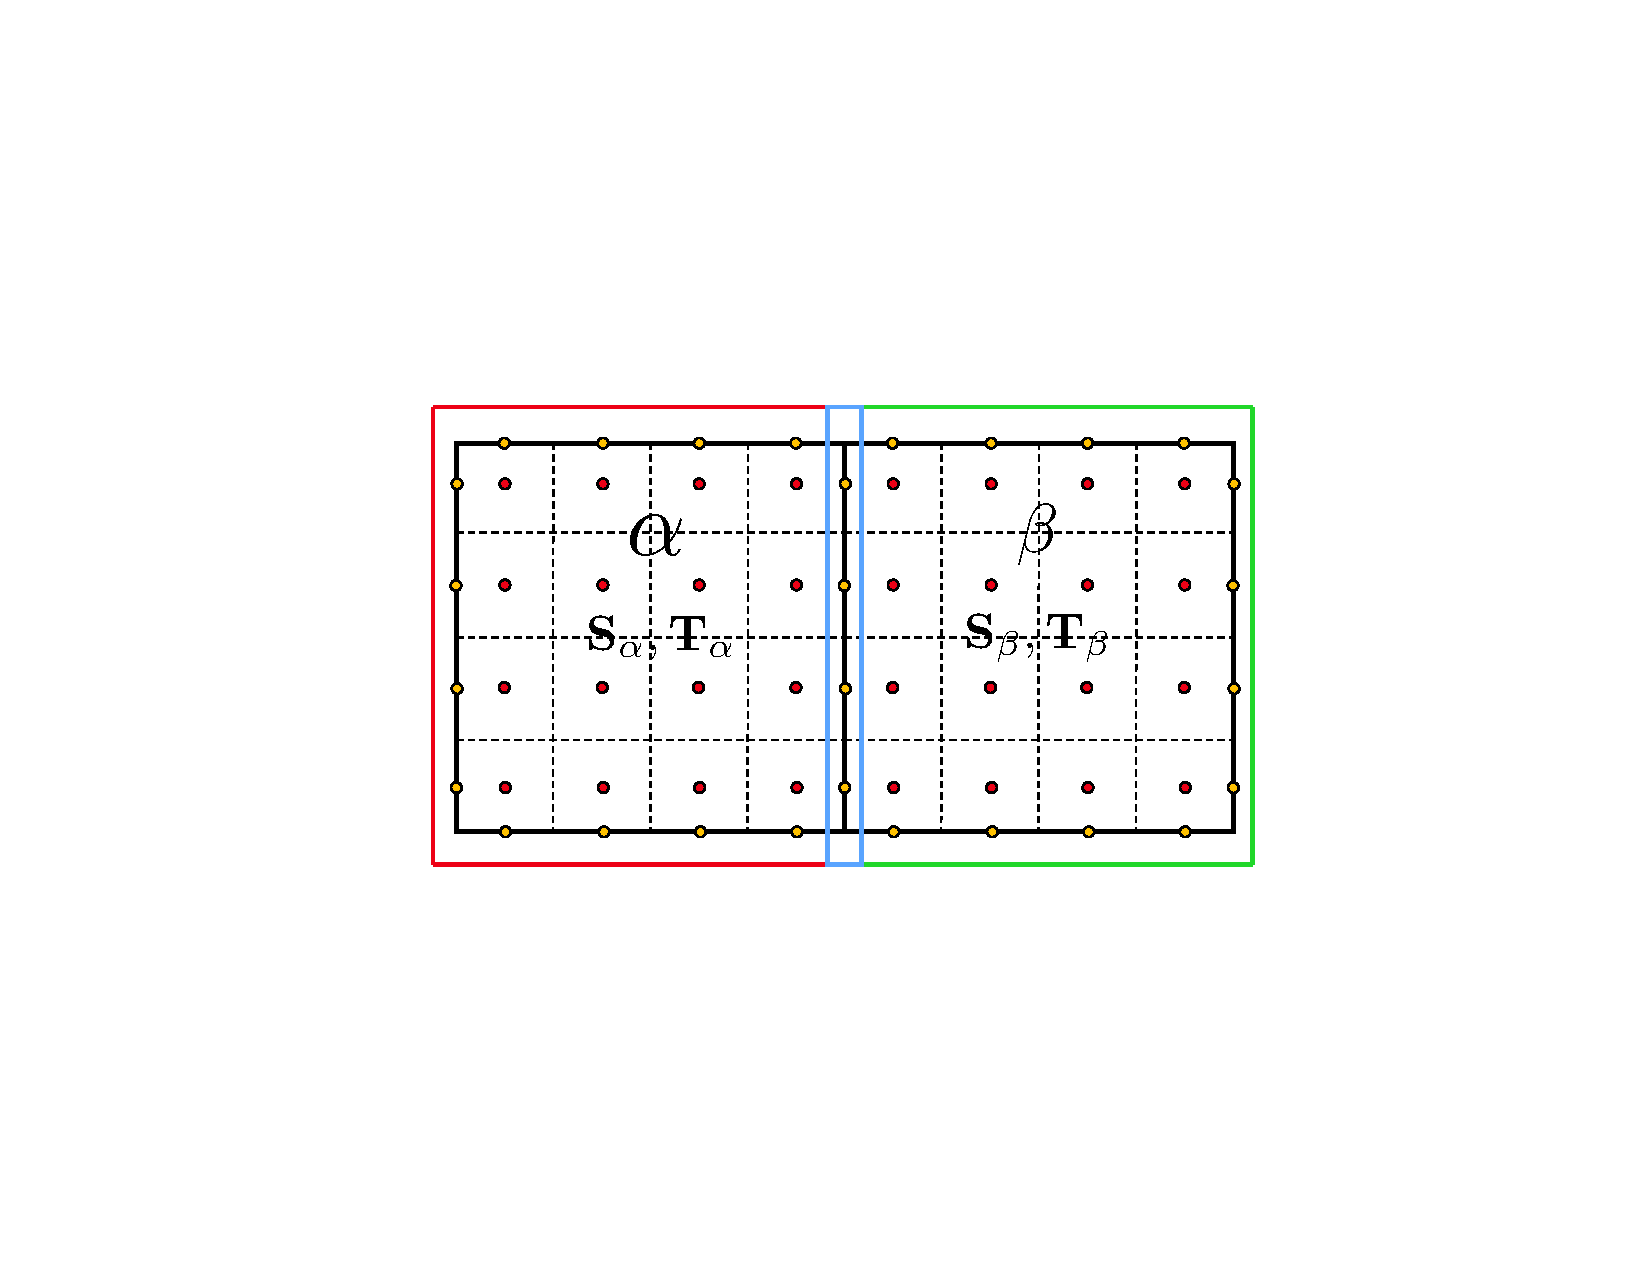
\includegraphics[width=\columnwidth]{figures/merge_figure.pdf}
    \caption{HPS Merge Operation. The merged patch $\Omega_{\tau}$ is the union of children $\Omega_{\alpha}$ and $\Omega_{\beta}$, i.e. $\Omega_{\tau} = \Omega_{\alpha} \cup \Omega_{\beta}$. Red, green, and blue nodes correspond to index sets $\textbf{I}_1$, $\textbf{I}_2$, and $\textbf{I}_3$, respectively. The merge operation eliminates the nodes on the interface of the children patches.}
    \label{fig:merge}
\end{figure}

With these definitions we can form the following linear systems by partioning according to the index sets:
\begin{align}
    \begin{bmatrix}
        \textbf{h}_1 \\
        \textbf{h}_3 \\
    \end{bmatrix} &=
    \begin{bmatrix}
        \textbf{T}_{1,1}^{\alpha} & \textbf{T}_{1,3}^{\alpha} \\
        \textbf{T}_{3,1}^{\alpha} & \textbf{T}_{3,3}^{\alpha} \\
    \end{bmatrix}
    \begin{bmatrix}
        \textbf{g}_1 \\
        \textbf{g}_3 \\
    \end{bmatrix} \\
    \begin{bmatrix}
        \textbf{h}_2 \\
        \textbf{h}_3 \\
    \end{bmatrix} &=
    \begin{bmatrix}
        \textbf{T}_{2,2}^{\beta} & \textbf{T}_{2,3}^{\beta} \\
        \textbf{T}_{3,2}^{\beta} & \textbf{T}_{3,3}^{\beta} \\
    \end{bmatrix}
    \begin{bmatrix}
        \textbf{g}_2 \\
        \textbf{g}_3 \\
    \end{bmatrix}.
\end{align}
The goal is to build merged operators $\textbf{S}^{\tau}$ and $\textbf{T}^{\tau}$ such that
\begin{align}
    \textbf{g}_3 &= \textbf{S}^{\tau}
    \begin{bmatrix}
        \textbf{g}_1 \\
        \textbf{g}_2 \\
    \end{bmatrix} \\
    \begin{bmatrix}
        \textbf{h}_1 \\
        \textbf{h}_2 \\
    \end{bmatrix} &=
    \textbf{T}^{\tau}
    \begin{bmatrix}
        \textbf{g}_1 \\
        \textbf{g}_2 \\
    \end{bmatrix}.
\end{align}
To accomplish this, eliminate $\textbf{h}_3$ and write the blocked linear system
\begin{align}
    \begin{bmatrix}
        \begin{matrix}
            \textbf{T}_{1,1}^{\alpha} & \textbf{0} \\
             \textbf{0} & \textbf{T}_{2,2}^{\beta} \\
        \end{matrix}
        & \vline &
        \begin{matrix}
            \textbf{T}_{1,3}^{\alpha} \\
            \textbf{T}_{2,3}^{\beta} \\
        \end{matrix} \\
        \hline
        \begin{matrix}
            \textbf{T}_{3,1}^{\alpha} & - \textbf{T}_{3,2}^{\beta}
        \end{matrix}
        & \vline &
        \begin{matrix}
            \textbf{T}_{3,3}^{\alpha} - \textbf{T}_{3,3}^{\beta}
        \end{matrix}
    \end{bmatrix}
    \begin{bmatrix}
        \textbf{g}_1 \\
        \textbf{g}_2 \\
        \hline
        \textbf{g}_3
    \end{bmatrix} =
    \begin{bmatrix}
        \textbf{h}_1 \\
        \textbf{h}_2 \\
        \hline
        \textbf{0} \\
    \end{bmatrix}
\end{align}
which tells us an expression for $\textbf{S}^{\tau}$ (last equation) and for $\textbf{T}^{\tau}$ by forming a Schur complement to eliminate $\textbf{g}_3$ as
\begin{align}
    \textbf{S}^{\tau} &= (\textbf{T}^{\alpha}_{3,3} - \textbf{T}^{\beta}_{3,3})^{-1} \big[ -\textbf{T}^{\alpha}_{3,1} \ \ \textbf{T}^{\beta}_{3,2} \big]
    \label{merge_S}
\end{align}
\begin{align}
    \textbf{T}^{\tau} &=
    \begin{bmatrix}
        \textbf{T}^{\alpha}_{1,1} & \textbf{0} \\
        \textbf{0} & \textbf{T}^{\beta}_{2,2} \\
    \end{bmatrix} +
    \begin{bmatrix}
        \textbf{T}^{\alpha}_{1,3} \\
        \textbf{T}^{\beta}_{2,3} \\
    \end{bmatrix}
    \textbf{S}^{\tau}
    \label{merge_T}
\end{align}
These are the general expressions for merging two local patches. These general expressions can be adapted to both horizontal and vertical merges by following the index sets defined above.

\subsubsection{Solve Stage: Applying the Solution Operator}

With the leaf level computations and the merging complete, the build stage forms a global solution operator $\textbf{S}_0$ corresponding to the mapping of parent level Dirichlet data (the original problem data) to interior data. The solve stage then applies the operator in a downwards pass through the tree. This is simply a matrix-vector multiplication given as
\begin{align}
    \textbf{u}_{int} = \textbf{S}^{\tau} \textbf{g}^{\tau}
\end{align}
for all patches $\tau = 0, 1, 2, ..., N_{patches} - 1$. This iterates down the tree mapping boundary data to interface data. On the leaf level, the operator maps boundary data to solution data in the entire leaf patch. Figure \ref{fig:solve} demonstrates this stage.

In terms of performance, this is where the HPS method (and direct methods in general) shine. Once the work to build the solution operator is done, applying it is fast and can be done for any number of problems and boundary conditions.

\subsubsection{A Note on Performance and Accuracy}

Now that we have the details of the HPS method, let's address how well it performs. Following the analysis in \cite{martinsson2015hierarchical} and \cite{gillman2014direct}, they show that the total cost of the build and solve stages is:
\begin{align}
    \text{Build Stage }& \approx N^{1.5} \\
    \text{Solve Stage }& \approx N \log N,
\end{align}
where $N = $ total number of discretization nodes. Regarding accuracy, both Martinsson and Gillman report that "the merge stage is exact when performed in exact arithmetic. The only approximation involved is the approximation of the solution on a leaf by its interpolating polynomial" (\cite{martinsson2015hierarchical}, \cite{gillman2014direct}). The leaf level computations are only as good as the accuracy of the solution operator. And the solve stage is simply applying the solution operator. So, we expect that the accuracy and convergence of the HPS method is as good as the leaf level solution operator. Further convergence analysis and theory are also in development.

\begin{figure}
    \centering
    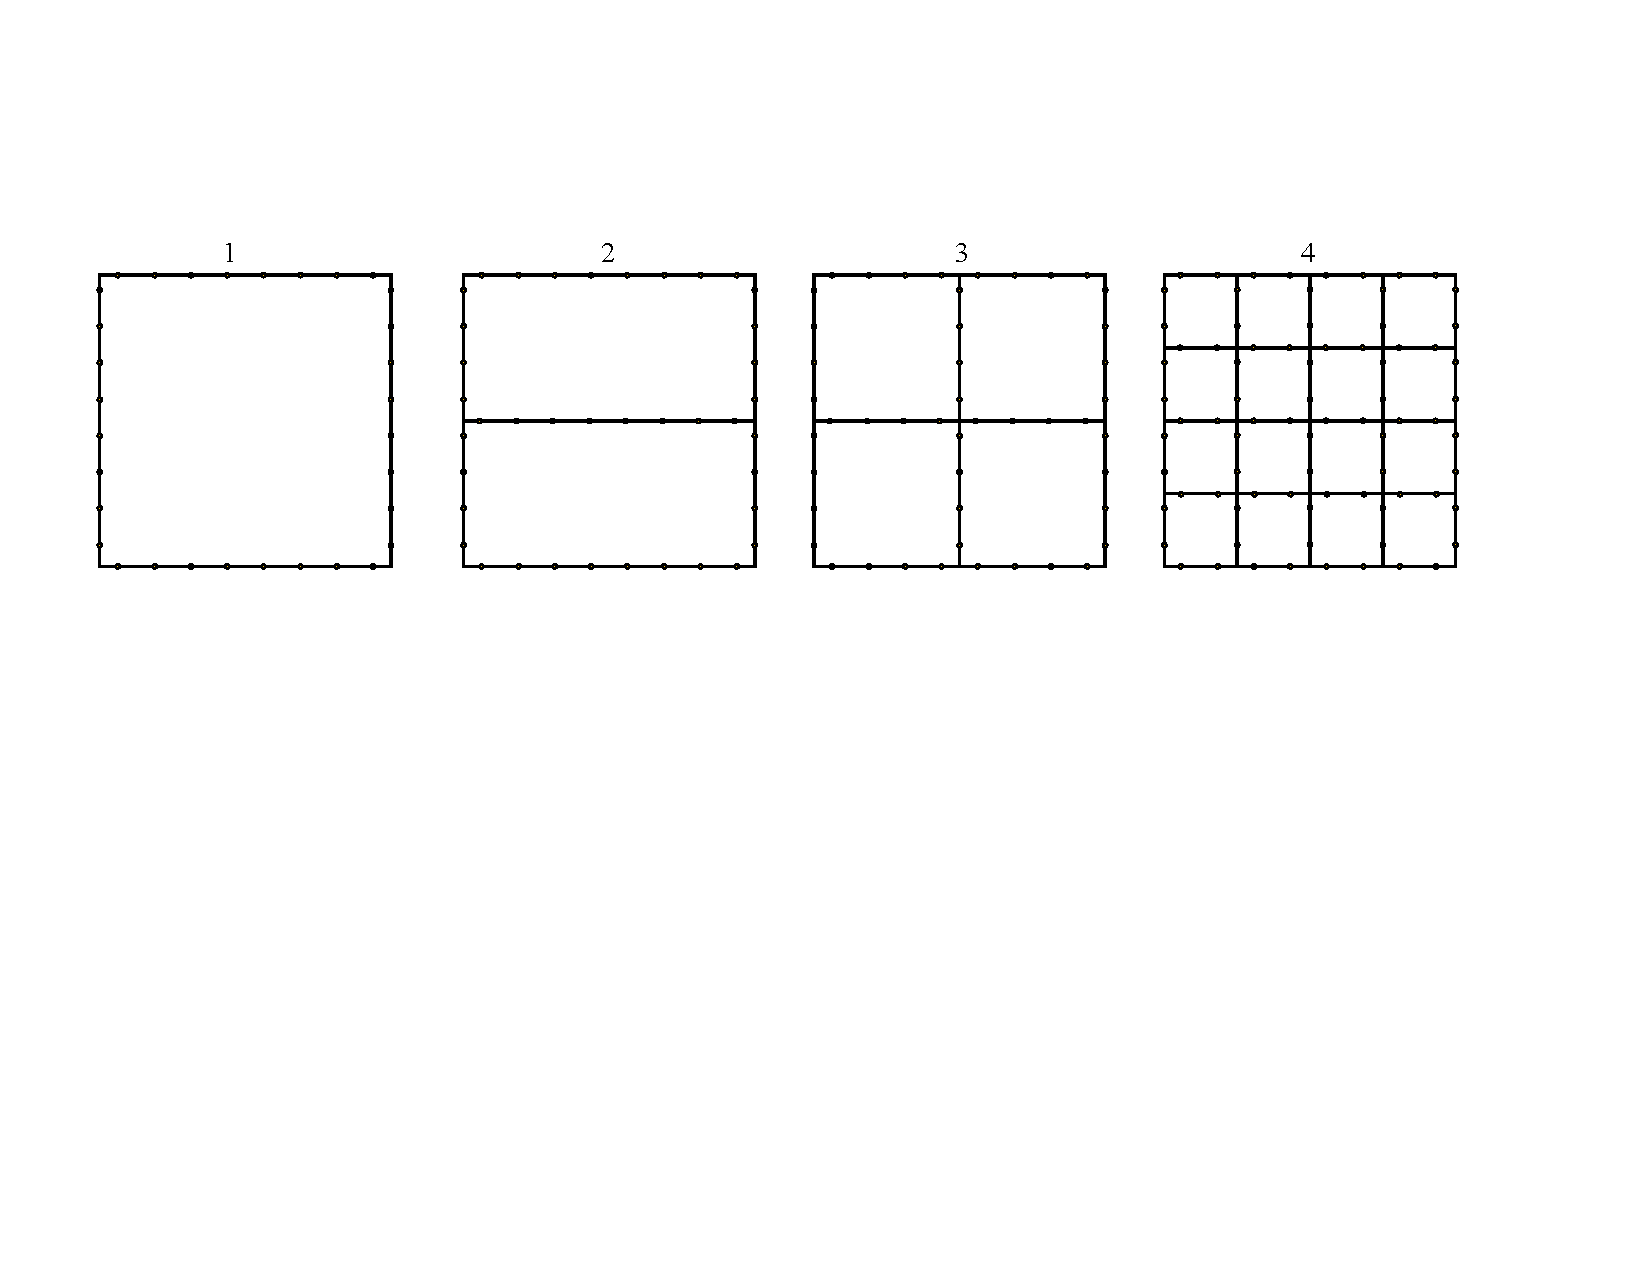
\includegraphics[width=\columnwidth]{figures/solve_figure.pdf}
    \caption{HPS Solve Stage. Once $\textbf{S}_0$ is formed, apply it to the top level Dirichlet data to get boundary (and solution) data on the interface of the children. Apply the patch solution operator down the tree until each leaf has it's local boundary information. Then apply the solution operator to get the solution data in the interior of each leaf.}
    \label{fig:solve}
\end{figure}

The HPS method, as detailed above, already shows promise and improvements towards fast, direct solvers, with a naive complexity of order $\mathcal{O}(N^{3/2})$. In \cite{gillman2014direct}, Gillman accelerates the work done in \cite{martinsson2015hierarchical} and describes how to achieve asymptotical performance of order $\mathcal{O}(N)$.

\subsection{Accelerating the Hierarchical Poincaré-Steklov Method}

As Gillman notes in \cite{gillman2014direct}, the most expensive part of the HPS algorithm is in the merge operation. At the top level, computing the merged operators involve dense matricies of $\mathcal{O}(N^{1/2}) \times \mathcal{O}(N^{1/2})$ for an overall cost of $\mathcal{O}(N^{3/2})$. It is possible to take advantage of the internal structure of these matricies to accelerate the matrix algebra. Gillman notes that the ``off-diagonal blocks of these matricies are to, high precision, rank deficient" and can be represented in a ``data-sparse" format called hierarchically block seperable (HBS) (\cite{gillman2014direct}). We will follow \cite{gillman2014direct} and \cite{gillman2012direct} to describe what it means to be HBS and how to use this property to apply inverses and operators.

\subsubsection{Hierarchically Block Seperable Matricies}

Let $\textbf{H}$ be an $mp \times mp$ matrix that is blocked into $p \times p$ blocks, each of size $m \times m$
\begin{align}
    \textbf{H} &=
    \begin{bmatrix}
        \textbf{D}_1     & \textbf{H}_{1,2} & \textbf{H}_{1,3} & ...    & \textbf{H}_{1,p} \\
        \textbf{H}_{2,1} & \textbf{D}_{2}   & \textbf{H}_{2,3} & ...    & \textbf{H}_{2,p} \\
        \textbf{H}_{3,1} & \textbf{H}_{3,2} & \textbf{D}_{3}   & ...    & \textbf{H}_{3,p} \\
        \vdots           & \vdots           & \vdots           & \ddots & \vdots           \\
        \textbf{H}_{p,1} & \textbf{H}_{p,2} & \textbf{H}_{p,3} & ...    & \textbf{D}_{p} \\
    \end{bmatrix}.
\end{align}
Gillman calls matrix $\textbf{H}$ ``block seperable" with ``block-rank" $k$ if for $\tau = 1,2,...,p$ there exists $m \times k$ matricies $\textbf{U}_{\tau}$ and $\textbf{V}_{\tau}$ such that each off-diagonal block $\textbf{H}_{\sigma, \tau}$ of $\textbf{H}$ admits the factorization
\begin{align}
    \textbf{H}_{\sigma, \tau} &= \textbf{U}_{\sigma} \tilde{\textbf{H}}_{\sigma, \tau} \textbf{V}_{\tau}^*.
\end{align}
If this holds, then the block seperable matrix $\textbf{H}$ admits the following block factorization
\begin{align}
    \textbf{H} &= \underline{\textbf{U}} \tilde{\textbf{H}} \underline{\textbf{V}}^* + \textbf{D},
\end{align}
where
\begin{align}
    \underline{\textbf{U}} &= \text{diag}(\textbf{U}_1, \textbf{U}_2, ..., \textbf{U}_p) \\
    \underline{\textbf{V}} &= \text{diag}(\textbf{V}_1, \textbf{V}_2, ..., \textbf{V}_p) \\
    \underline{\textbf{D}} &= \text{diag}(\textbf{D}_1, \textbf{D}_2, ..., \textbf{D}_p),
\end{align}
and
\begin{align}
    \tilde{\textbf{H}} &=
    \begin{bmatrix}
        \textbf{0}       & \tilde{\textbf{H}_{1,2}} & \tilde{\textbf{H}_{1,3}} & ...    & \tilde{\textbf{H}_{1,p}} \\
        \tilde{\textbf{H}_{2,1}} & \textbf{0}       & \tilde{\textbf{H}_{2,3}} & ...    & \tilde{\textbf{H}_{2,p}} \\
        \tilde{\textbf{H}_{3,1}} & \tilde{\textbf{H}_{3,2}} & \textbf{0}       & ...    & \tilde{\textbf{H}_{3,p}} \\
        \vdots           & \vdots           & \vdots           & \ddots & \vdots           \\
        \tilde{\textbf{H}_{p,1}} & \tilde{\textbf{H}_{p,2}} & \tilde{\textbf{H}_{p,3}} & ...    & \textbf{0}       \\
    \end{bmatrix}
\end{align}

Perhaps the most important property of these HBS matricies is that not only is $\textbf{H}$ HBS, but $\tilde{\textbf{H}}$ is HBS also. As well as the middle matrix of it's factorization, and so on. This property is what allows us to both store HBS matricies in a ``data-sparse" format and compute/apply inverses and matricies fast.

\subsubsection{Inverting and Applying HBS Matricies}
\label{subsub:applyHBS}

Taking advantage of the properties of HBS matrices, Gillman shows in \cite{gillman2012direct} how to use HBS matricies. She details in \cite{gillman2012direct}: Algorithm 2 how to perform a matrix-vector product with an HBS matrix, in \cite{gillman2012direct}: Algorithm 3 how to invert an HBS matrix, and in \cite{gillman2012direct}: Algorithm 4 how to apply an inverse of an HBS matrix. Gillman also states the complexity of building and applying an HBS inverse to be order $\mathcal{O}(N)$ and provides the theorem therein.

\subsubsection{Extensions to HBS Matricies}

Due to the low-rank structure of HBS matricies, further optimizations are possible. Xia in \cite{xia2013randomized} extend the topic of randomized matricies to HBS matricies to achieve further speed up and better data storage.

\subsubsection{Using HBS Matricies in the Direct Solver}

To bring the discussion back to the HPS method, we look at how we can use HBS matricies and randomized matrix math to accelerate the HPS direct solver. Xia in \cite{xia2013randomized} applies her randomized sparse solver to various sparse matricies that arise from various applications such as PDE discretizations and graph theory. Gillman in \cite{gillman2014direct} uses HBS matricies to accelerate the HPS method. As we are interested in direct solvers for elliptic PDES, we will follow Gillman's extension of HBS matricies to the HPS method.

Gillman starts by showing that the merge operations for $\textbf{S}^{\tau}$ and $\textbf{T}^{\tau}$ are formed from HBS matricies. Once this is shown, we can look at the merge operation can be accelerated using HBS operators. The solution operator in \ref{merge_S} is formed by 1) adding HBS matricies $\textbf{T}_{3,3}^{\alpha}$ and $-\textbf{T}_{3,3}^{\beta}$, 2) inverting this result, and 3) applying the HBS inverse to either of the low-rank matricies $\textbf{T}_{3,1}^{\alpha}$ and $\textbf{T}_{3,2}^{\beta}$.

Forming the DtN operator is done in a similar manner: 1) Form the matrix products $\textbf{T}_{1,3}^{\alpha} \textbf{S}^{\tau}$ and $\textbf{T}_{2,3}^{\beta} \textbf{S}^{\tau}$ using HBS algorithms, then 2) perform a low-rank update to the block diagonal matrix in \ref{merge_T}.

Applying the solution operator in the build stage can also take advantage of HBS algorithms, and is simply an HBS matrix-vector product down the tree.

The algorithms mentioned in \ref{subsub:applyHBS} from \cite{gillman2012direct} are the methods that can be used to perform this linear algebra in a fast manner.

Now, in practice, it is more efficient to simply use dense matrix algebra on the lower levels of the tree. At some point however, the matricies become large enough that the use and overhead of the HBS matrix math is smaller than simple dense matrix math, thus achieving speed up compared to an all dense matrix math implementation.

\subsection{Extensions of the Hierarchical Poincaré-Steklov Method}

The HPS method as detailed above, in both it's naive order $\mathcal{O}(N^{3/2})$ implementation or it's accelerated order $\mathcal{O}(N)$ implementation, provides a revolutionary direct method to solve elliptic PDEs. As such, there have already been various extensions and applications of the HPS method, and we will detail a few of them here.

\subsubsection{Non-Homogenous Elliptic PDEs}

The HPS method builds a global solution operator $\textbf{S}$ and DtN operator $\textbf{T}$. This works for both non-homogenous and homogenous BVPs like in \ref{bvp}. However, in order to solve non-homogenous BVPs, some additional information needs to be computed and stored in the build and solve stage. This stems from the superposition principle for elliptic PDEs.

The idea in solving non-homogenous BVPs is to split the solution $u$ of \ref{bvp} into a particular and homogenous solution $u = w + \phi$. This is the same as solving the following two BVPs:
\begin{align}
    \begin{cases}
        \mathcal{A} w(\textbf{x}) = f(\textbf{x}), &\textbf{x} \in \Omega \\
        u(\textbf{x}) = 0, &\textbf{x} \in \partial \Omega = \Gamma
    \end{cases}
\end{align}
and
\begin{align}
    \begin{cases}
        \mathcal{A} \phi(\textbf{x}) = 0, &\textbf{x} \in \Omega \\
        u(\textbf{x}) = g(\textbf{x}), &\textbf{x} \in \partial \Omega = \Gamma
    \end{cases}.
\end{align}

Applying the same discretization as before (either spectral, finite difference/finite volume grid, etc.), we now need to keep track of two new vectors of information: $\textbf{w}$ and $\hat{\textbf{w}}$ which correspond to the local particular solution and the derivative of the local particular solution, respectively. $\textbf{w}$ can be found by applying the solution operator or function to a problem with zero boundary conditions, and $\hat{\textbf{w}}$ can be found by applying a derivative operator to $\textbf{w}$.

The merge operator then must also compute a merged $\hat{\textbf{w}}$ done with the following expression:
\begin{align}
    \hat{\textbf{w}} &=
    \begin{bmatrix}
        \hat{\textbf{w}}_1^{\alpha} \\
        \hat{\textbf{w}}_2^{\beta} \\
    \end{bmatrix} +
    \begin{bmatrix}
        \textbf{T}_{1,3}^{\alpha} \\
        \textbf{T}_{2,3}^{\beta} \\
    \end{bmatrix}
    (\textbf{T}_{3,3}^{\alpha} - \textbf{T}_{3,3}^{\beta})^{-1} (\hat{\textbf{w}}_3^{\beta} - \hat{\textbf{w}}_3^{\alpha})
\end{align}

While these additional computations do not increase the asymptotical performance of the HPS method, it does significantly increase the amount of storage required due to the need to store additional vectors. Gillman and Martinsson detail the non-homogenous HPS method in both their presentations of the HPS method in \cite{gillman2014direct}, \cite{martinsson2015hierarchical}, and \cite{martinsson2019fast}.

\subsubsection{The Adaptive Hierarchical Poincaré-Steklov Method}

One of the major advantages to using the HPS method is it's hierarchical discretization. While the original presentation of the HPS method only considers uniform meshes, the HPS method can also be implemented on an adaptive mesh. This type of meshing, and the performance associated with the HPS method, make it of particular interest when solving the Serre-Green-Nagdhi model as most finite volume codes employ dynamic (as in changes with each time step), adaptive meshing. This is the case for ForestClaw, which we will use for the hyperbolic part of the Serre-Green-Nagdhi solver \cite{calhoun2017forestclaw}.

Geldermans et al. in \cite{geldermans2019adaptive} extend the HPS method to work on non-uniform meshes. Their primary modification is in using a different tensor basis that is more efficient and stable in order to provide accurate interpolation between non-uniform mesh boundaries. As the HPS method already allows for a recursive splitting and merging, the main problem to address in an adaptive setting is how to handle coarse-fine boundaries. As Geldermans et al. use a spectral discretization of Chebyshev nodes, they use spectral interpolation methods in order to handle merging of patches that do not lie on the same level. They present an adaptive HPS algorithm for solving elliptic PDEs and show that they can still achieve fast performance and accurate results.

\subsubsection{The Ultraspherical Spectral Element Method}

The ultraspherical spectral element method (ultraSEM) presented by Fortunato et al. is another highly practical extension of the HPS method. In \cite{fortunato2020ultraspherical}, they apply their ultraspherical spectral element method from \cite{olver2013fast} to the HPS method. Namely, by using spectral discretization on leaf nodes that can also be mapped quadrilaterals and triangles, and using the HPS method for merging and building global operators, they use the HPS method on unstructured meshes. In addition, this demonstrates that the idea of the HPS method of hierarchically merging patches can be applied to any type of solution for BVPs, whether it be a finite difference, finite volume, finite element, spectral element method or others.
